\documentclass[11pt]{article}

% This first part of the file is called the PREAMBLE. It includes
% customizations and command definitions. The preamble is everything
% between \documentclass and \begin{document}.

\usepackage[margin=1in]{geometry}  % set the margins to 1in on all sides

\usepackage{graphicx}              % to include figures
\usepackage{amsmath}               % great math stuff
\usepackage{amsfonts}              % for blackboard bold, etc
\usepackage{amsthm}                % better theorem environments

\usepackage{dcolumn}
\usepackage{dsfont}
\usepackage{array}
\usepackage{booktabs}
\usepackage{soul}
\usepackage{mathrsfs}
\usepackage{enumerate}
\usepackage{multicol}
\usepackage[makeroom]{cancel}
\usepackage{xcolor}
\usepackage{tikz}
\usepackage{pdfpages}

% various theorems, numbered by section

\newtheorem{thm}{Theorem}[section]
\newtheorem{lem}[thm]{Lemma}
\newtheorem{prop}[thm]{Proposition}
\newtheorem{cor}[thm]{Corollary}
\newtheorem{conj}[thm]{Conjecture}
\newtheorem{exer}[thm]{Exercise}

\DeclareMathOperator{\id}{id}

\newcommand{\bd}[1]{\mathbf{#1}}  % for bolding symbols
\newcommand{\RR}{\mathbb{R}}      % for Real numbers
\newcommand{\ZZ}{\mathbb{Z}}      % for Integers
\newcommand{\col}[1]{\left[\begin{matrix} #1 \end{matrix} \right]}
\newcommand{\comb}[2]{\binom{#1^2 + #2^2}{#1+#2}}
\newcommand{\overfrac}[2]{\genfrac{}{}{0pt}{}{#1}{#2}}

\renewcommand{\thesubsection}{\thesection.\alph{subsection}}

\everymath{\displaystyle}

\setlength\parindent{0pt}

\usepackage{setspace}

\begin{document}
\begin{multicols}{2}
  \phantom{hello}\vspace{0.01\baselineskip}
  \phantom{hello}\vspace{0.01\baselineskip}
  {\large Assignment 4}\\
  \begin{flushright}
    Mikhail Gaerlan (914437675)\\
    21 April 2017\\
    STA 243 Lee
  \end{flushright}
\end{multicols}
\vspace{-2.3\baselineskip}

\hrulefill

\section{}

$\int_a^bf(x)h(x)dx$ can be approximated by
\begin{eqnarray*}
  \hat{\mu}_{MC}&=&\frac{1}{n}\sum_{i=1}^nh(X_i)\\
  \textrm{Var}\left(\hat{\mu}_n\right)&=&\frac{1}{n}\sum_{i=1}^n\left(h\left(X_i\right)-\hat{\mu}_{MC}\right)^2
\end{eqnarray*}
where $X_i$ is sampled from $f(x)$.

\subsection{$\int_0^1x^2dx$}
\begin{eqnarray*}
  f(x)&=&\mathds{1}_{[0,1]}(x)\\
  h(x)&=&x^2\\
  n&=&1000
\end{eqnarray*}
\begin{center}
  \begin{tabular}{ r@{\hspace{.1cm}}c@{\hspace{.1cm}}r@{\hspace{.0cm}}c@{\hspace{.0cm}}l }
    $\hat{\mu}_n$&$=$&$0$&$.$&$33910520$\\
    $\textrm{Var}\left(\hat{\mu}_n\right)$&$=$&$0$&$.$&$08896713$
  \end{tabular}
\end{center}

\subsection{$\int_0^1\int_{-2}^2x^2\cos\left(xy\right)dxdy$}
\begin{eqnarray*}
  f(x,y)&=&\frac{1}{4}\mathds{1}_{[-2,2]}(x)\mathds{1}_{[0,1]}(y)\\
  h(x,y)&=&4x^2\cos\left(xy\right)\\
  n&=&1000
\end{eqnarray*}
\begin{center}
  \begin{tabular}{ r@{\hspace{.1cm}}c@{\hspace{.1cm}}r@{\hspace{.0cm}}c@{\hspace{.0cm}}l }
    $\hat{\mu}_n$&$=$&$3$&$.$&$501649$\\
    $\textrm{Var}\left(\hat{\mu}_n\right)$&$=$&$13$&$.$&$390987$
  \end{tabular}
\end{center}

\subsection{$\int_0^\infty\frac{3}{4}x^4e^{-x^3/4}dx$}
\begin{eqnarray*}
  f(x)&=&\frac{1}{4}\mathds{1}_{[0,\infty)}(x)e^{-x/4}\\
  h(x)&=&3x^4e^{-x^3/4+x/4}\\
  n&=&1000
\end{eqnarray*}
\begin{center}
  \begin{tabular}{ r@{\hspace{.1cm}}c@{\hspace{.1cm}}r@{\hspace{.0cm}}c@{\hspace{.0cm}}l }
    $\hat{\mu}_n$&$=$&$2$&$.$&$188157$\\
    $\textrm{Var}\left(\hat{\mu}_n\right)$&$=$&$12$&$.$&$954084$
  \end{tabular}
\end{center}

\section{$ I=\frac{1}{\sqrt{2\pi}}\int_1^2e^{-x^2/2}dx$}

\begin{eqnarray*}
  f(x)&=&\mathds{1}_{[1,2]}\\
  h(x)&=&\frac{1}{\sqrt{2\pi}}e^{-x^2/2}\\
  g(x)&=&\frac{1}{\sqrt{2\pi\nu^2}}e^{-(x-1.5)^2/2\nu^2}\\
  n&=&10000
\end{eqnarray*}
\begin{center}
  \begin{tabular}{ cr@{\hspace{.1cm}}c@{\hspace{.1cm}}r@{\hspace{.0cm}}c@{\hspace{.0cm}}l cr@{\hspace{.1cm}}c@{\hspace{.1cm}}r@{\hspace{.0cm}}c@{\hspace{.0cm}}lcr@{\hspace{.1cm}}c@{\hspace{.1cm}}r@{\hspace{.0cm}}c@{\hspace{.0cm}}l}
    $\nu = 0.1$,&$\hat{I}_n$&$=$&$0$&$.$&$1169773$,&$\nu = 1$,&$\hat{I}_n$&$=$&$0$&$.$&$13391863$,&$\nu = 10$,&$\hat{I}_n$&$=$&$0$&$.$&$1344222$\\
               &$\textrm{Var}\left(\hat{I}_n\right)$&$=$&$3$&$.$&$1721584$&&$\textrm{Var}\left(\hat{I}_n\right)$&$=$&$0$&$.$&$03766775$&&$\textrm{Var}\left(\hat{I}_n\right)$&$=$&$0$&$.$&$5202285$\\
  \end{tabular}
\end{center}

\begin{table*}[h]
  \begin{center}
    \renewcommand{\arraystretch}{1.5}
    \begin{tabular}{| >{\centering\arraybackslash}m{2.1in} |  >{\centering\arraybackslash}m{2.1in} |  >{\centering\arraybackslash}m{2.1in}|}
      \hline
      $\nu=0.1$&$\nu=1$&$\nu=10$\\\hline
      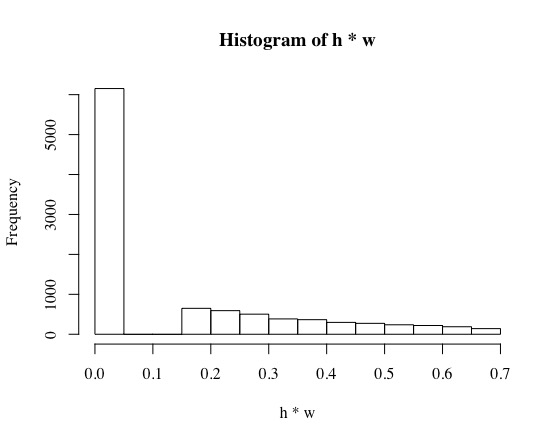
\includegraphics[width=1\linewidth,height=0.18\textheight]{plot2-1-1}&
      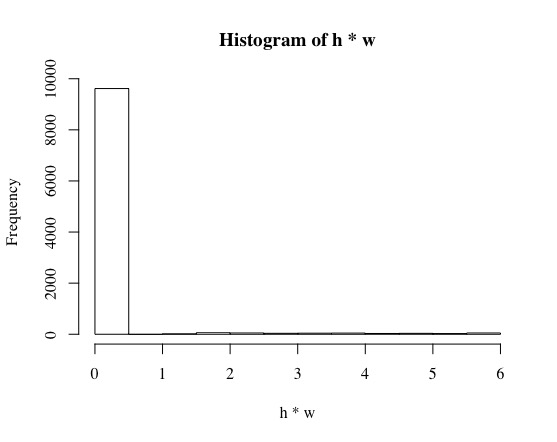
\includegraphics[width=1\linewidth,height=0.18\textheight]{plot2-1-2}&
      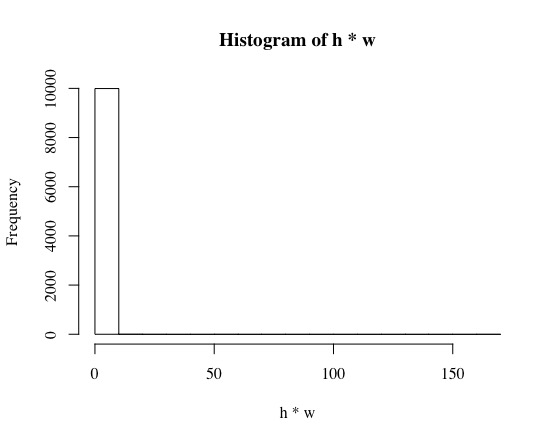
\includegraphics[width=1\linewidth,height=0.18\textheight]{plot2-1-3}\\\hline
    \end{tabular}
  \end{center}
\end{table*}

\section{$I=\int_0^1\frac{1}{1+x}dx$}
\subsection{}

\begin{eqnarray*}
  f(x)&=&\mathds{1}_{[0,1]}\\
  h(x)&=&\frac{1}{1+x}\\
  n&=&1500
\end{eqnarray*}
\begin{center}
  \begin{tabular}{ r@{\hspace{.1cm}}c@{\hspace{.1cm}}r@{\hspace{.0cm}}c@{\hspace{.0cm}}l }
    $\hat{I}_{MC}$&$=$&$0$&$.$&$69635548$\\
    $\textrm{Var}\left(\hat{I}_{MC}\right)$&$=$&$0$&$.$&$02066273$
  \end{tabular}
\end{center}

\subsection{}

\begin{eqnarray*}
  b &=& \frac{\textrm{Cov}\left(\hat{I}_{MC},\hat{\theta}_{MC}\right)}{\textrm{Var}\left(\hat{\theta}_{MC}\right)},\qquad \hat{\theta}_{MC}=\frac{1}{n}\sum_{i=1}^{n}c\left(U_i\right)\\
  \textrm{Cov}\left(\hat{I}_{MC},\hat{\theta}_{MC}\right)&=&\frac{1}{n-1}\sum_{i=1}^n\left[h\left(U_i\right)-\hat{I}_{MC}\right]\left[c\left(U_i\right)-\hat{\theta}_{MC}\right]\\
  \textrm{Var}\left(\hat{\theta}_{MC}\right)&=&\frac{1}{n-1}\sum_{i=1}^n\left(c\left(U_i\right)-\hat{\theta}_{MC}\right)^2
\end{eqnarray*}
\begin{eqnarray*}
  E\left\{c\left(U\right)\right\} &=& \int_0^1\left(1+x\right)dx\\
                                  &=& \left.x+\frac{1}{2}x^2\,\right|_0^1=\frac{3}{2}
\end{eqnarray*}

\begin{center}
  \begin{tabular}{ r@{\hspace{.1cm}}c@{\hspace{.1cm}}r@{\hspace{.0cm}}c@{\hspace{.0cm}}l }
    $b$&$=$&$-0$&$.$&$4793439$\\
    $\hat{I}_{CV}$&$=$&$0$&$.$&$6944337896$\\
    $\textrm{Var}\left(\hat{I}_{CV}\right)$&$=$&$0$&$.$&$0006408379$
  \end{tabular}
\end{center}

\subsection{}

The variance for $\hat{I}_{CV}$ is 2 orders of magnitude smaller than for $\hat{I}_{MC}$.
\begin{center}
  \begin{tabular}{ r@{\hspace{.1cm}}c@{\hspace{.1cm}}r@{\hspace{.0cm}}c@{\hspace{.0cm}}l }
    $\textrm{Var}\left(\hat{I}_{MC}\right)$&$=$&$0$&$.$&$02066273$\\
    $\textrm{Var}\left(\hat{I}_{CV}\right)$&$=$&$0$&$.$&$0006408379$
  \end{tabular}
\end{center}

\subsection{}

Define two control variates $c_1(x),c_2(x)$ so
\begin{eqnarray*}
  \hat{I}_{CV}=\frac{1}{n}\sum_{i=1}^nh\left(U_i\right)-b_1\left[\frac{1}{n}\sum_{i=1}^nc_1\left(U_i\right)-E\left\{c_1\left(U\right)\right\}\right]-b_2\left[\frac{1}{n}\sum_{i=1}^nc_2\left(U_i\right)-E\left\{c_2\left(U\right)\right\}\right]\\
  \textrm{Var}\left(\hat{I}_{CV}\right)=\textrm{Var}\left(\hat{I}_{MC}\right)+b_1^2\textrm{Var}\left(\hat{\theta}_{1MC}\right)+b_2^2\textrm{Var}\left(\hat{\theta}_{2MC}\right)-2b_1\textrm{Cov}\left(\hat{I}_{MC},\hat{\theta}_{1MC}\right)-\\2b_2\textrm{Cov}\left(\hat{I}_{MC},\hat{\theta}_{2MC}\right)-2b_1b_2\textrm{Cov}\left(\hat{\theta}_{1MC},\hat{\theta}_{2MC}\right)\phantom{\textrm{Var}\left(\hat{I}_{MC}\right)}
\end{eqnarray*}
where the optimal $b_1,b_2$ are
\begin{eqnarray*}
  b_1&=&\frac{\textrm{Cov}\left(\hat{\theta}_{1MC},\hat{\theta}_{2MC}\right)\textrm{Cov}\left(\hat{I}_{MC},\hat{\theta}_{2MC}\right)+\textrm{Cov}\left(\hat{I}_{MC},\hat{\theta}_{1MC}\right)\textrm{Var}\left(\hat{\theta}_{2MC}\right)}{\textrm{Var}\left(\hat{\theta}_{1MC}\right)\textrm{Var}\left(\hat{\theta}_{2MC}\right)-\left(\textrm{Cov}\left(\hat{\theta}_{1MC},\hat{\theta}_{2MC}\right)\right)^2}\\
  b_2&=&\frac{\textrm{Cov}\left(\hat{\theta}_{1MC},\hat{\theta}_{2MC}\right)\textrm{Cov}\left(\hat{I}_{MC},\hat{\theta}_{1MC}\right)+\textrm{Cov}\left(\hat{I}_{MC},\hat{\theta}_{2MC}\right)\textrm{Var}\left(\hat{\theta}_{1MC}\right)}{\textrm{Var}\left(\hat{\theta}_{1MC}\right)\textrm{Var}\left(\hat{\theta}_{2MC}\right)-\left(\textrm{Cov}\left(\hat{\theta}_{1MC},\hat{\theta}_{2MC}\right)\right)^2}
\end{eqnarray*}

\section{}

\subsection{}\label{anova}

$H_0$: If $\mu_j=\sum_{i=1}^ny_{ij}$, then all the $\mu_j$'s are the same.\\
$H_a$: $\exists\,i,j $ such that $\mu_i\neq \mu_j$\\
\\
Simulate the experiment from by generating $e_{ij}$ and thus a set of data $y_{ij}$. Then compute the average of all the $\mu_j$'s. Repeat 998 times. Generate 1 more average of the $\mu_j$'s. If the last $\mu_j$ is among the smallest 2.5\% or largest 2.5\%, then reject the null hypothesis.

\subsection{}

Similar to Problem \ref{anova} except repeat the entire process for various distributions for $e_{ij}$.

\section{}

\subsection{}

\begin{figure}[h!]
\begin{center}
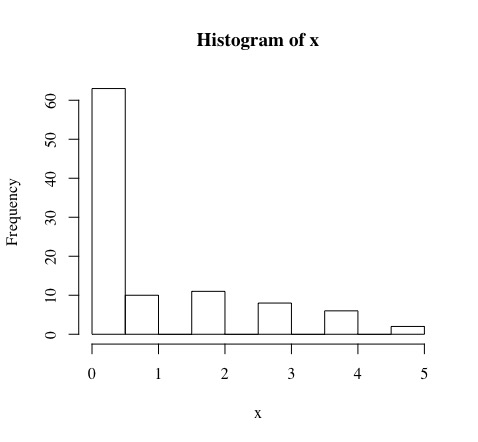
\includegraphics[height=0.3\textheight,width=0.45\linewidth]{plot5-a}
\end{center}
\label{initial}
\end{figure}

\subsection{}

\subsubsection{}

\begin{eqnarray*}
  f\left(\lambda\,|\,p,\mathbf{r},\mathbf{x}\right)&=&\frac{b^a\lambda^{a-1}e^{-b\lambda}}{\Gamma\left(a\right)}\prod_{i=1}^n\frac{e^{-\lambda r_i}\left(\lambda r_i\right)^{x_i}}{x_i!}p^{r_i}\left(1-p\right)^{1-r_i}\\
                                                   &=&\frac{b^a\lambda^{a-1}e^{-b\lambda}}{\Gamma\left(a\right)}e^{\lambda\Sigma_i r_i}\lambda^{\Sigma_i x_i}\prod_{i=1}^n\frac{r_i^{x_i}}{x_i!}p^{r_i}(1-p)^{1-r_i}\\
                                                   &=&\frac{b^a\lambda^{\left(a+\Sigma_i x_i\right)-1}e^{-\left(b+\Sigma_i r_i\right)\lambda}}{\Gamma\left(a\right)}\sum_{i=1}^n\frac{r_i^{x_i}}{\Gamma\left(x_i\right)}p^{r_i}\left(1-p\right)^{1-r_i}\\
                                                   &\vdots&\\
                                                   &\stackrel{?}{=}&\frac{\left(b+\Sigma_i r_i\right)^{\left(a+\Sigma_i x_i\right)}\lambda^{\left(a+\Sigma_i x_i\right)-1}e^{-\left(b+\Sigma_i r_i\right)\lambda}}{\Gamma\left(a+\Sigma_i x_i\right)}\\
  \left(\lambda\,|\,p,\mathbf{r},\mathbf{x}\right)&\sim&\textrm{Gamma}\left(a+\Sigma_i x_i,b+\Sigma_i r_i\right)
\end{eqnarray*}

\subsubsection{}

\begin{eqnarray*}
  f\left(p\,|\,\lambda,\mathbf{r},\mathbf{x}\right)&=&\frac{b^a\lambda^{a-1}e^{-b\lambda}}{\Gamma\left(a\right)}\prod_{i=1}^n\frac{e^{-\lambda r_i}\left(\lambda r_i\right)^{x_i}}{x_i!}p^{r_i}\left(1-p\right)^{1-r_i}\\
                                                   &\vdots&\\
                                                   &\stackrel{?}{=}&\frac{\Gamma\left(\left(1+\Sigma_i r_i\right)+\left(n+1-\Sigma_i r_i\right)\right)}{\Gamma\left(1+\Sigma_i r_i\right)\Gamma\left(n+1-\Sigma_i r_i\right)}x^{\left(1+\Sigma_i r_i\right)-1}\left(1-x\right)^{\left(n+1-\Sigma_i r_i\right)-1}\\
  \left(p\,|\,\lambda,\mathbf{r},\mathbf{x}\right)&\sim&\textrm{Beta}\left(1+\Sigma_i r_i,n+1-\Sigma_i r_i\right)
\end{eqnarray*}

\subsubsection{}

\begin{eqnarray*}
  f\left(\mathbf{r}\,|\,\lambda,p,\mathbf{x}\right)&=&\frac{b^a\lambda^{a-1}e^{-b\lambda}}{\Gamma\left(a\right)}\prod_{i=1}^n\frac{e^{-\lambda r_i}\left(\lambda r_i\right)^{x_i}}{x_i!}p^{r_i}\left(1-p\right)^{1-r_i}\\
                                                   &\vdots&\\
  f\left(r_i\,|\,\lambda,p,\mathbf{x}\right)&\stackrel{?}{=}&\left(\frac{pe^{-\lambda}}{pe^{-\lambda}+\left(1-p\right)I_{x_i=0}}\right)^{r_i}\left(1-\left(\frac{pe^{-\lambda}}{pe^{-\lambda}+\left(1-p\right)I_{x_i=0}}\right)\right)^{1-r_i}\\
  \left(r_i\,|\,\lambda,p,\mathbf{x}\right)&\sim&\textrm{Bernoulli}\left(\frac{pe^{-\lambda}}{pe^{-\lambda}+\left(1-p\right)I_{x_i=0}}\right)
\end{eqnarray*}

\subsection{}

\section{}

$X_0 = 1$. Sample $Y_i\sim\textrm{Gamma}\left(X_{i-1},\beta\right)$ and $U_i\sim \textrm{Unif}\left(0,1\right)$. To assess the accuracy, 100 sets of samples for each beta were found. The means $\mu_{\beta,j}(X),\mu_{\beta,j}(1/X), 1\leq j\leq 100$ of each set was determined. Then $\bar{\mu}_\beta(X)$, $\bar{\mu}_\beta(1/X)$ was found to be the means of $\{\mu_{\beta,1}(X_i),\ldots,\mu_{\beta,100}(X)\}$, $\{\mu_{\beta,1}(1/X),\ldots,\mu_{\beta,100}(1/X)\}$ and $\sigma_\beta^2(X),\sigma_\beta^2(1/X)$ was determined to be the mean and variance.
\begin{equation*}
  E(Z)=\sqrt{\frac{\theta_2}{\theta_1}}\approx 1.15470054\quad\textrm{and}\quad E\left(\frac{1}{Z}\right)=\sqrt{\frac{\theta_1}{\theta_2}}+\frac{1}{2\theta_2}\approx 1.11602540
\end{equation*}
\begin{center}
  \begin{tabular}{ cr@{\hspace{.1cm}}c@{\hspace{.1cm}}r@{\hspace{.0cm}}c@{\hspace{.0cm}}l cr@{\hspace{.1cm}}c@{\hspace{.1cm}}r@{\hspace{.0cm}}c@{\hspace{.0cm}}lcr@{\hspace{.1cm}}c@{\hspace{.1cm}}r@{\hspace{.0cm}}c@{\hspace{.0cm}}l}
    &$\beta$&$=$&$0$&$.$&$5$&&$\beta$&$=$&$1$&$.$&$0$&&$\beta$&$=$&$2$&$.$&$0$\\
    &$\bar{\mu}_\beta(X)$&$=$&$1$&$.$&$14311467$&&$\bar{\mu}_\beta(X)$&$=$&$1$&$.$&$15240804$&&$\bar{\mu}_\beta(X)$&$=$&$1$&$.$&$14157197$\\
    &$\sigma_\beta^2(X)$&$=$&$0$&$.$&$00401173$&&$\sigma_\beta^2(X)$&$=$&$0$&$.$&$00225613$&&$\sigma_\beta^2(X)$&$=$&$0$&$.$&$00463643$\\
                  &$\bar{\mu}_\beta(1/X)$&$=$&$1$&$.$&$11463973$&&$\bar{\mu}_\beta(1/X)$&$=$&$1$&$.$&$11431215$&&$\bar{\mu}_\beta(1/X)$&$=$&$1$&$.$&$112364733$\\
                  &$\sigma_\beta^2(1/X)$&$=$&$0$&$.$&$00220111$&&$\sigma_\beta^2(1/X)$&$=$&$0$&$.$&$00254056$&&$\sigma_\beta^2(1/X)$&$=$&$0$&$.$&$00564459$\\
  \end{tabular}
\end{center}

\begin{table*}[h]
  \begin{center}
    \renewcommand{\arraystretch}{1.5}
    \begin{tabular}{| >{\centering\arraybackslash}m{2.1in} |  >{\centering\arraybackslash}m{2.1in} |  >{\centering\arraybackslash}m{2.1in}|}
      \hline
      $\beta=0.5$&$\beta=1$&$\beta=2$\\\hline
      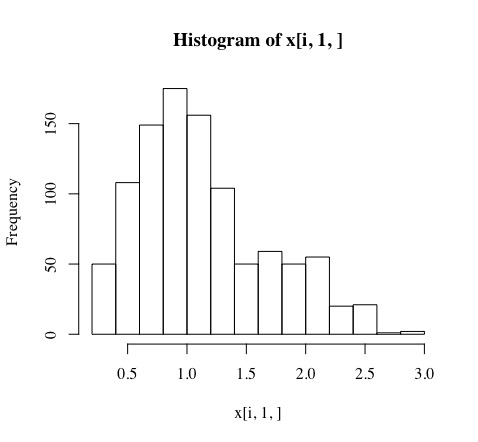
\includegraphics[width=1\linewidth,height=0.18\textheight]{plot6-1}&
      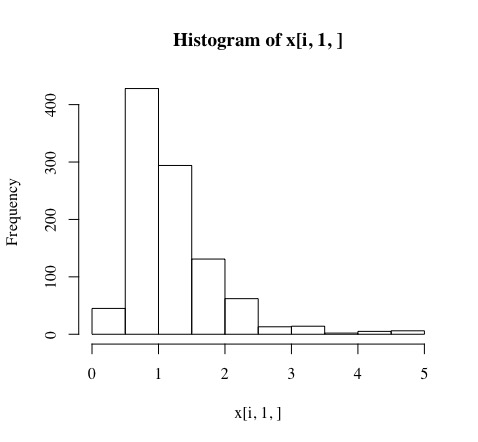
\includegraphics[width=1\linewidth,height=0.18\textheight]{plot6-2}&
      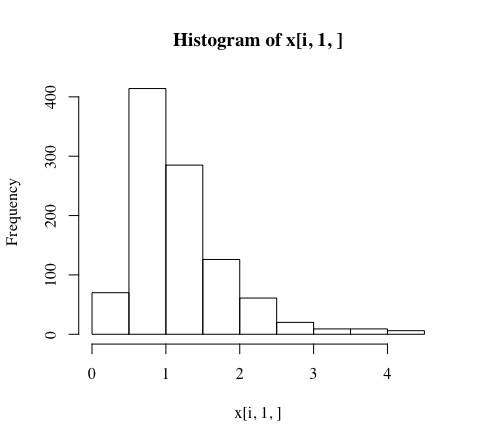
\includegraphics[width=1\linewidth,height=0.18\textheight]{plot6-3}\\\hline
    \end{tabular}
  \end{center}
\end{table*}

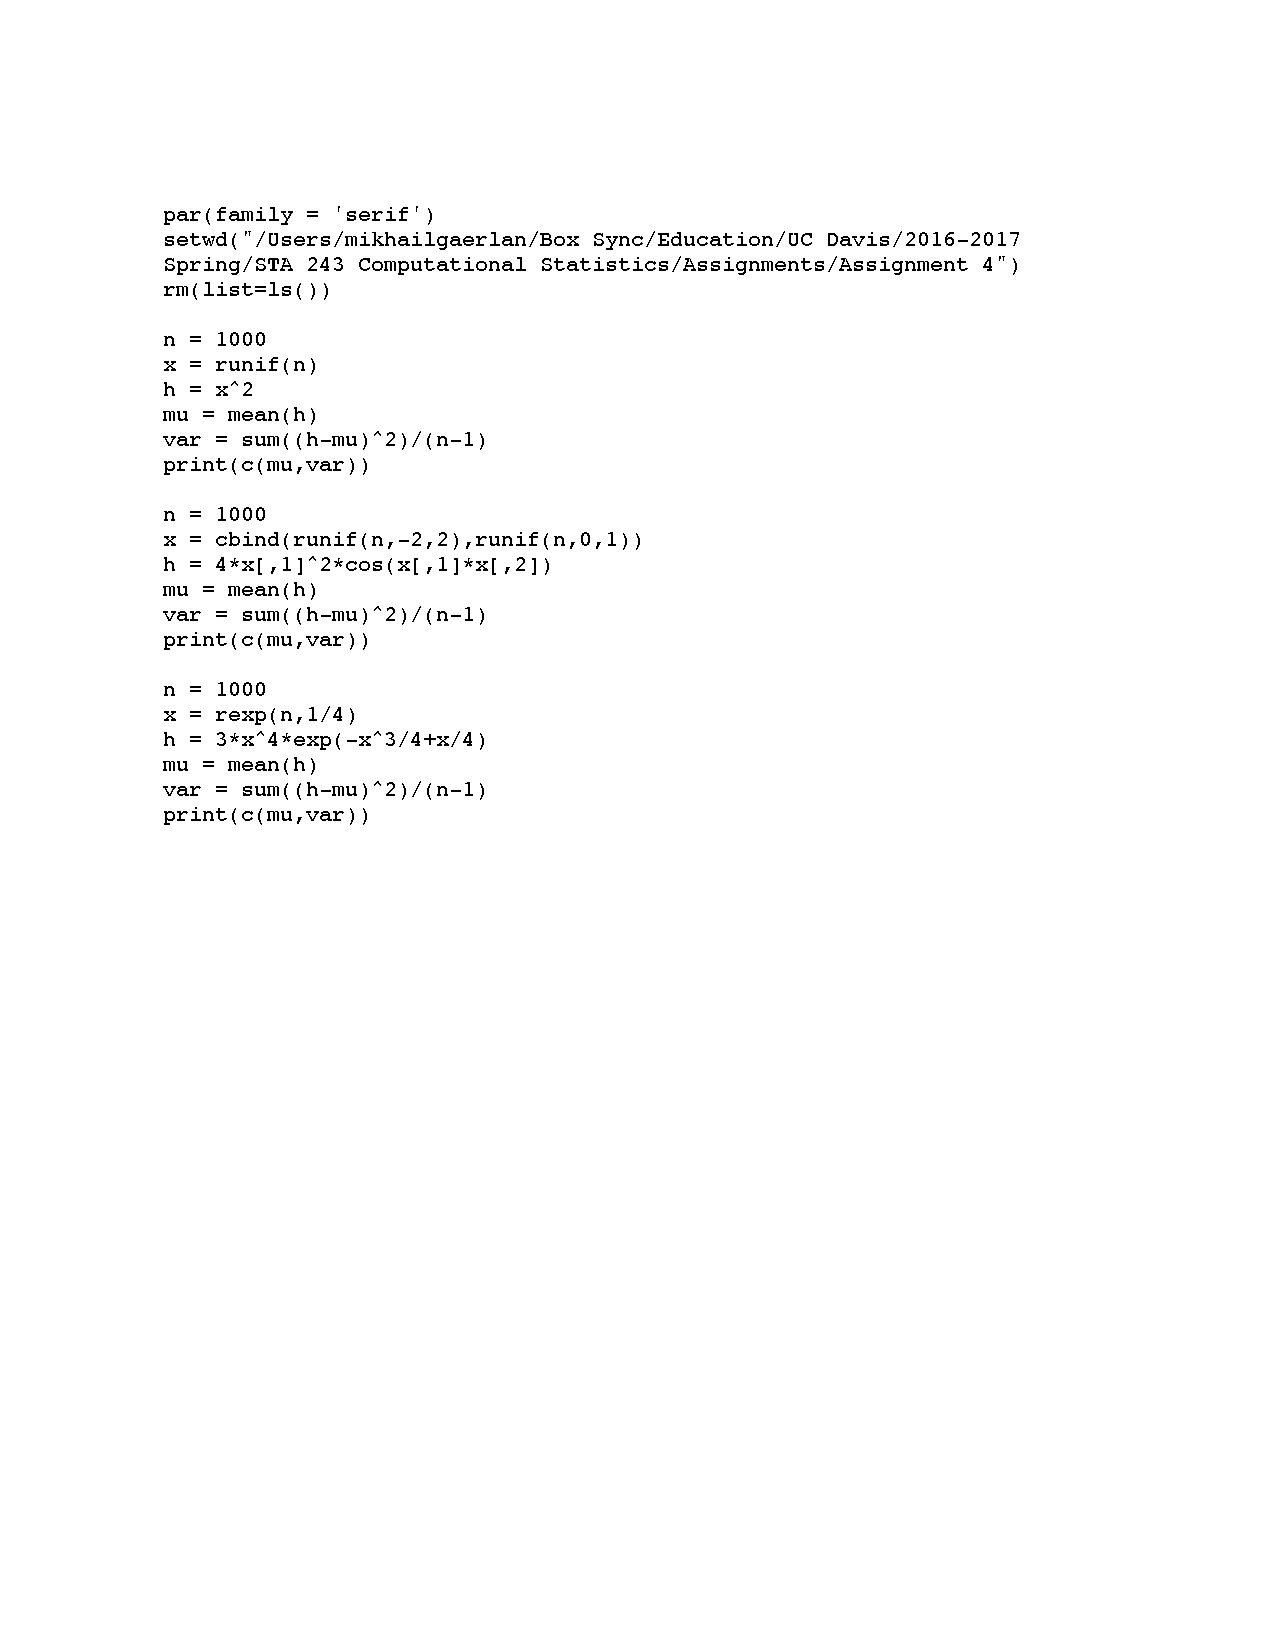
\includepdf[pages={1-1}]{code1.pdf}
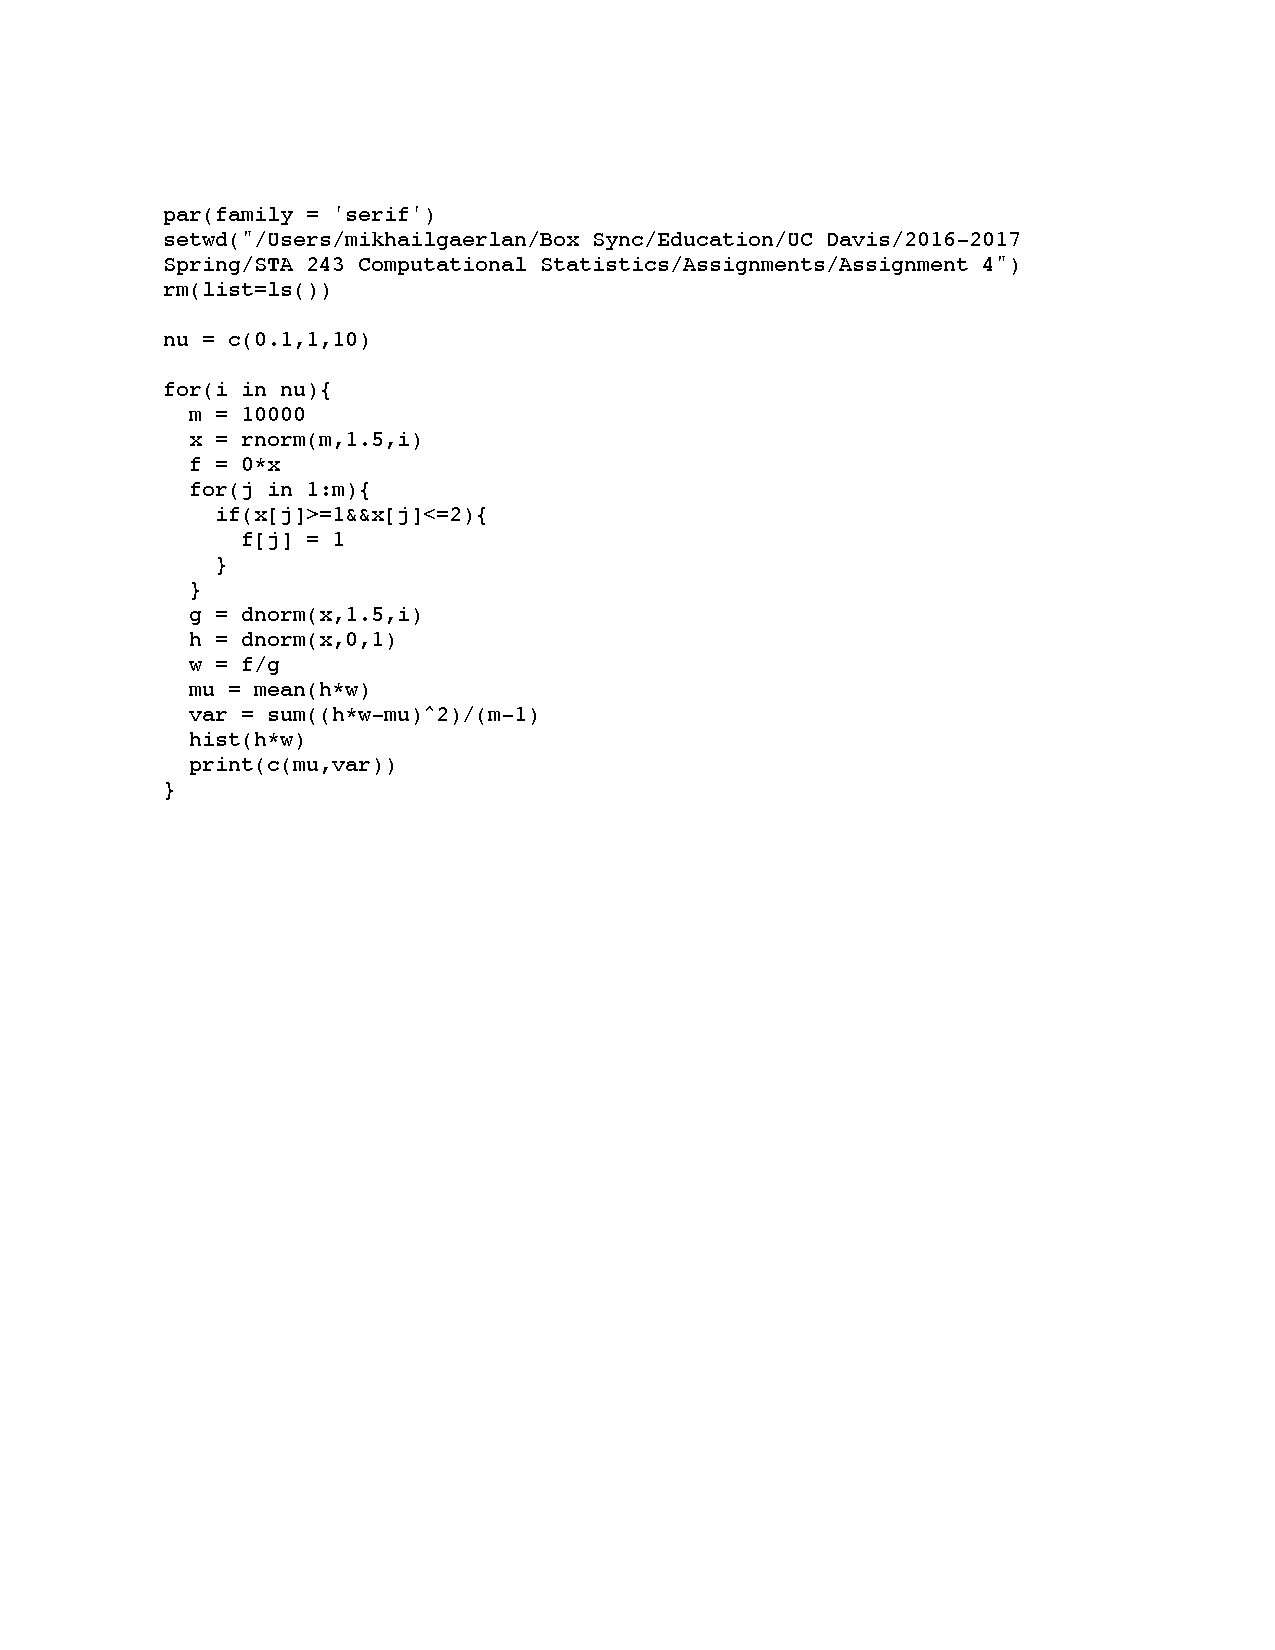
\includepdf[pages={1-1}]{code2.pdf}
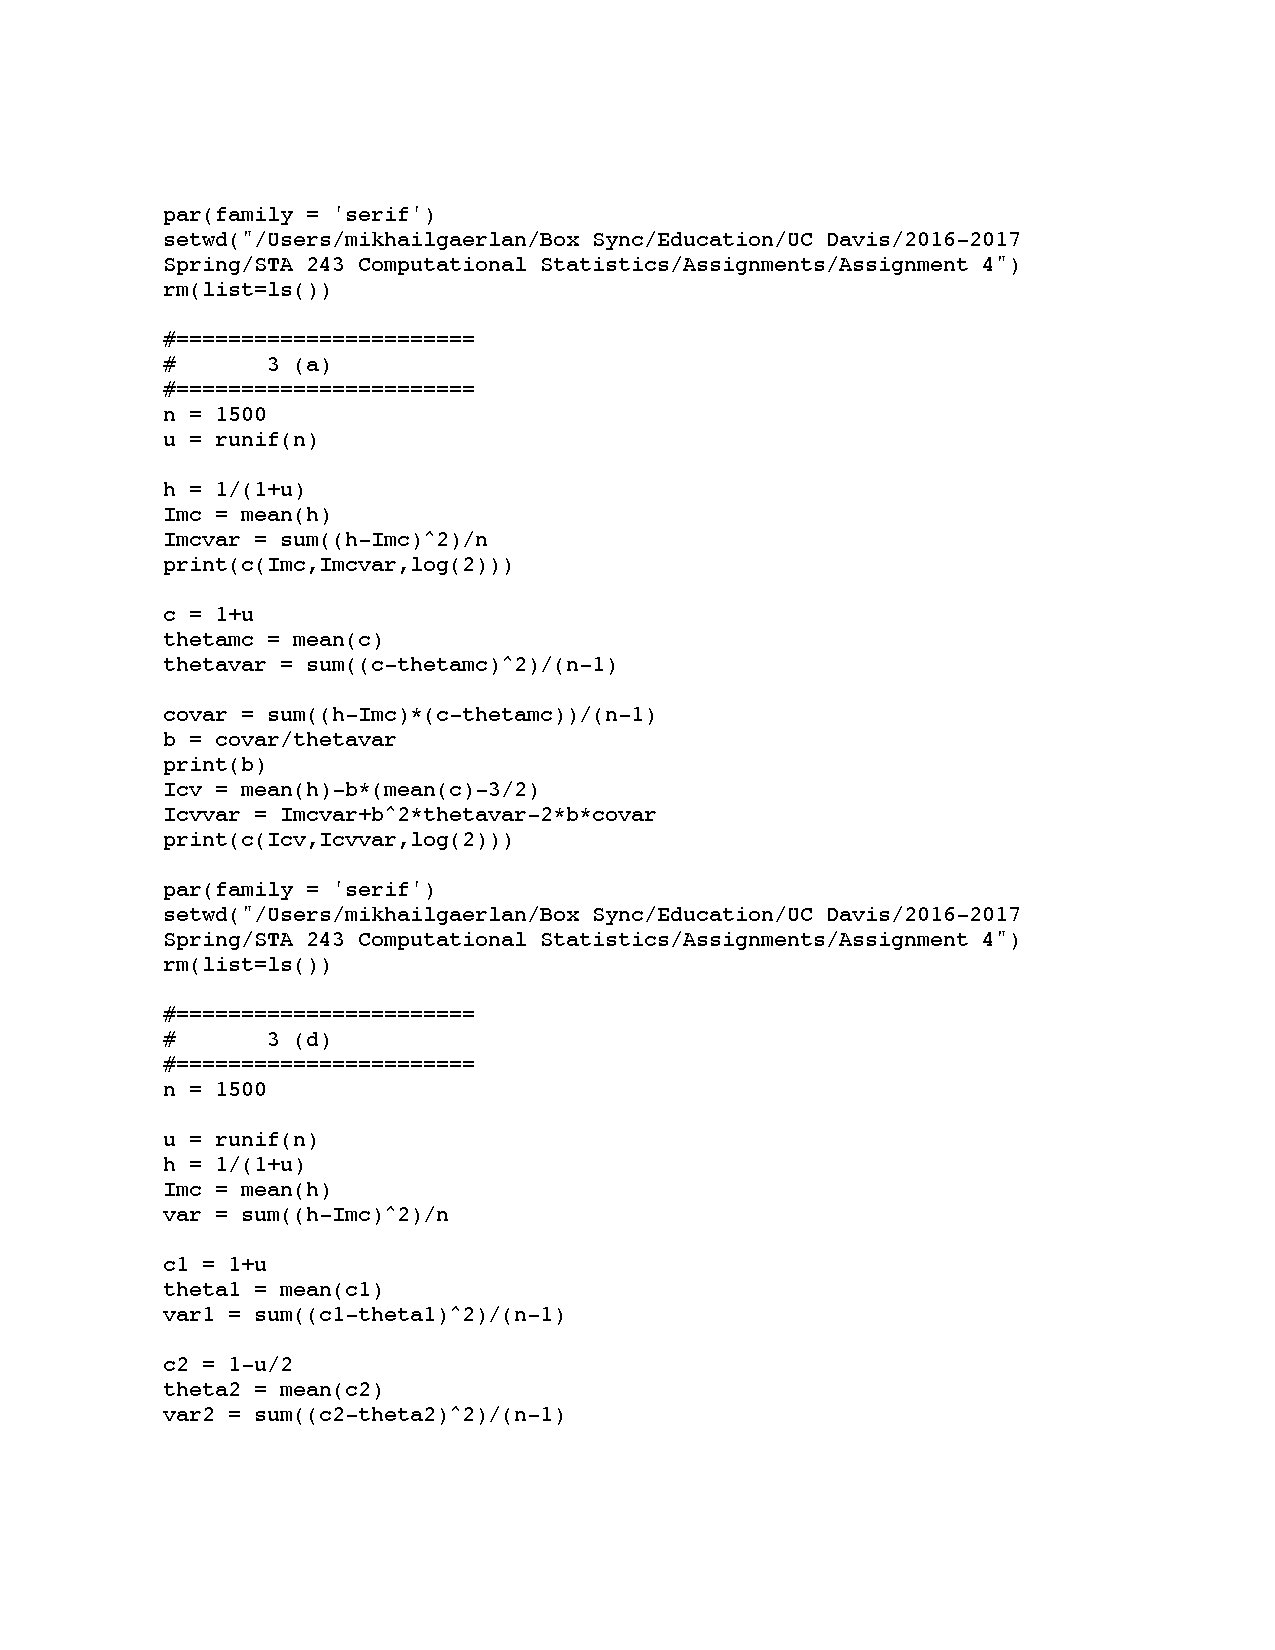
\includepdf[pages={1-2}]{code3.pdf}
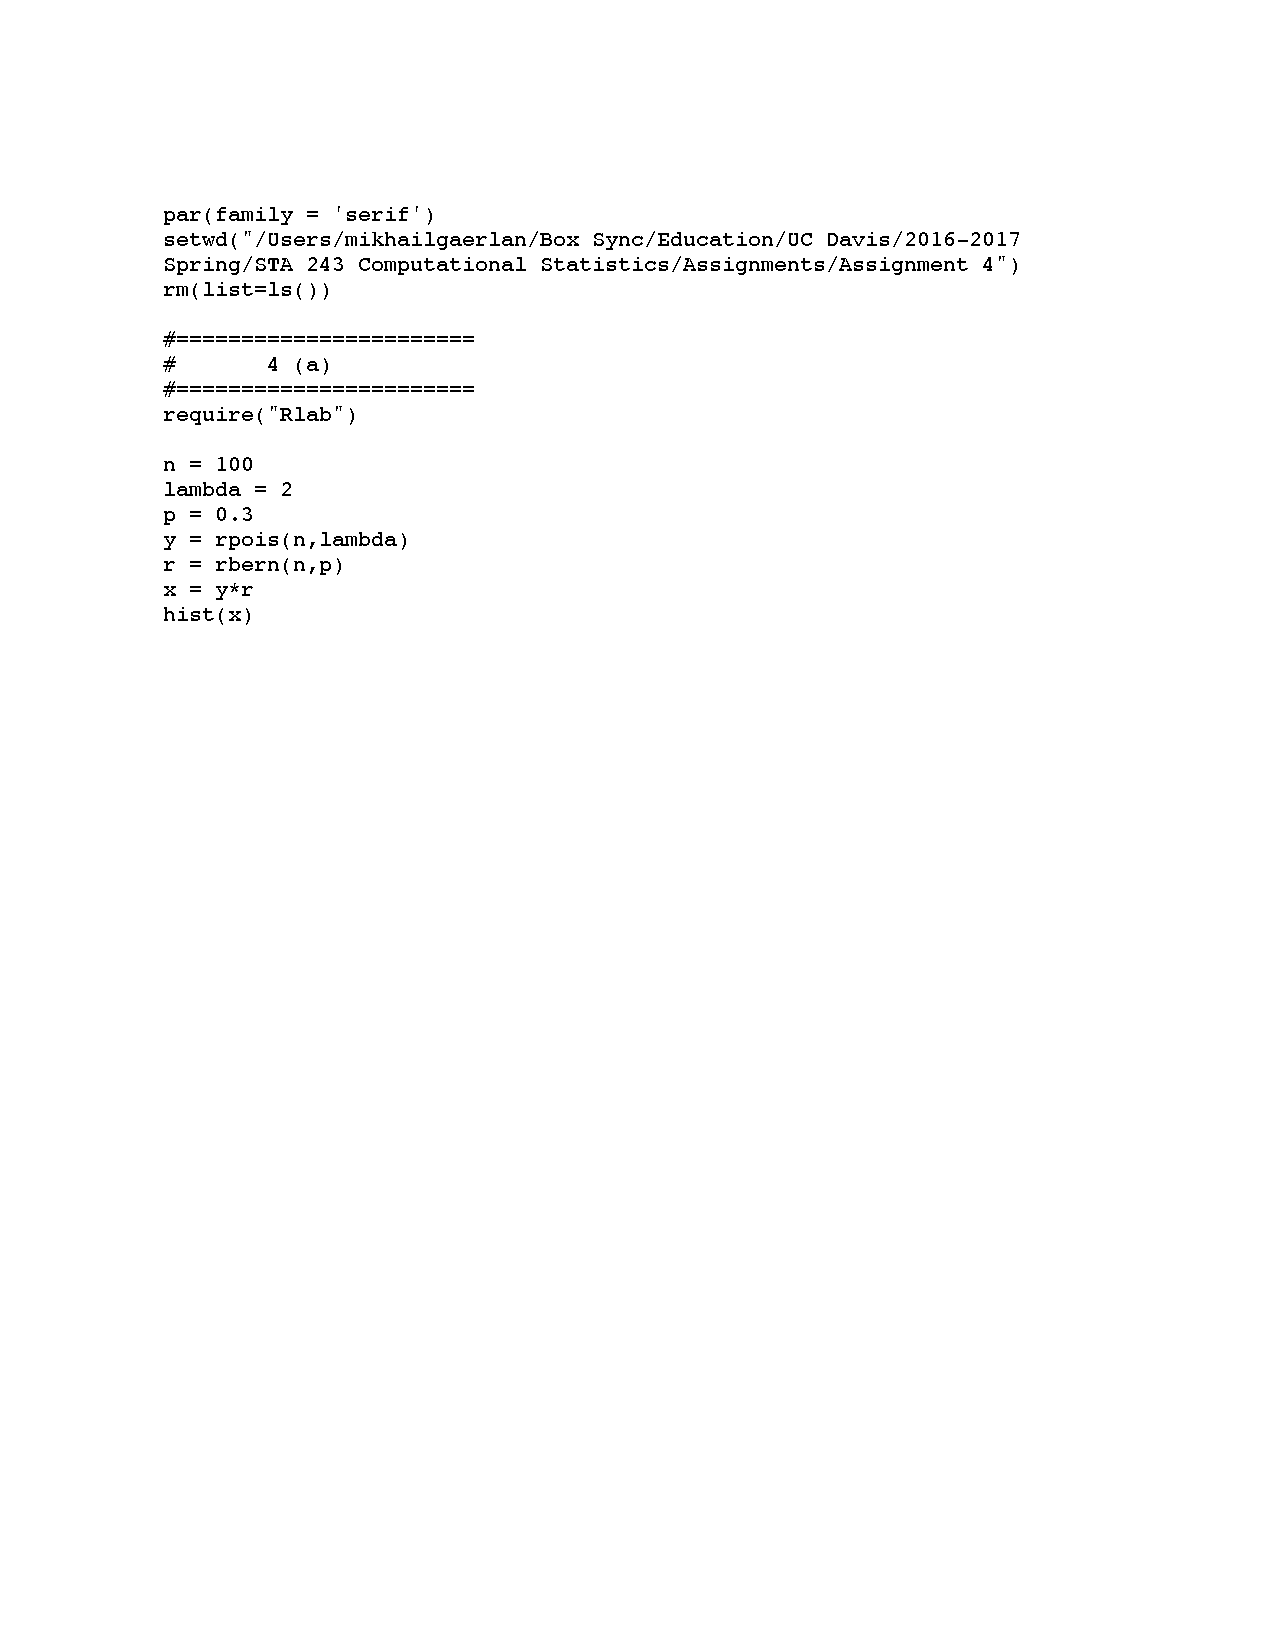
\includepdf[pages={1-1}]{code5.pdf}
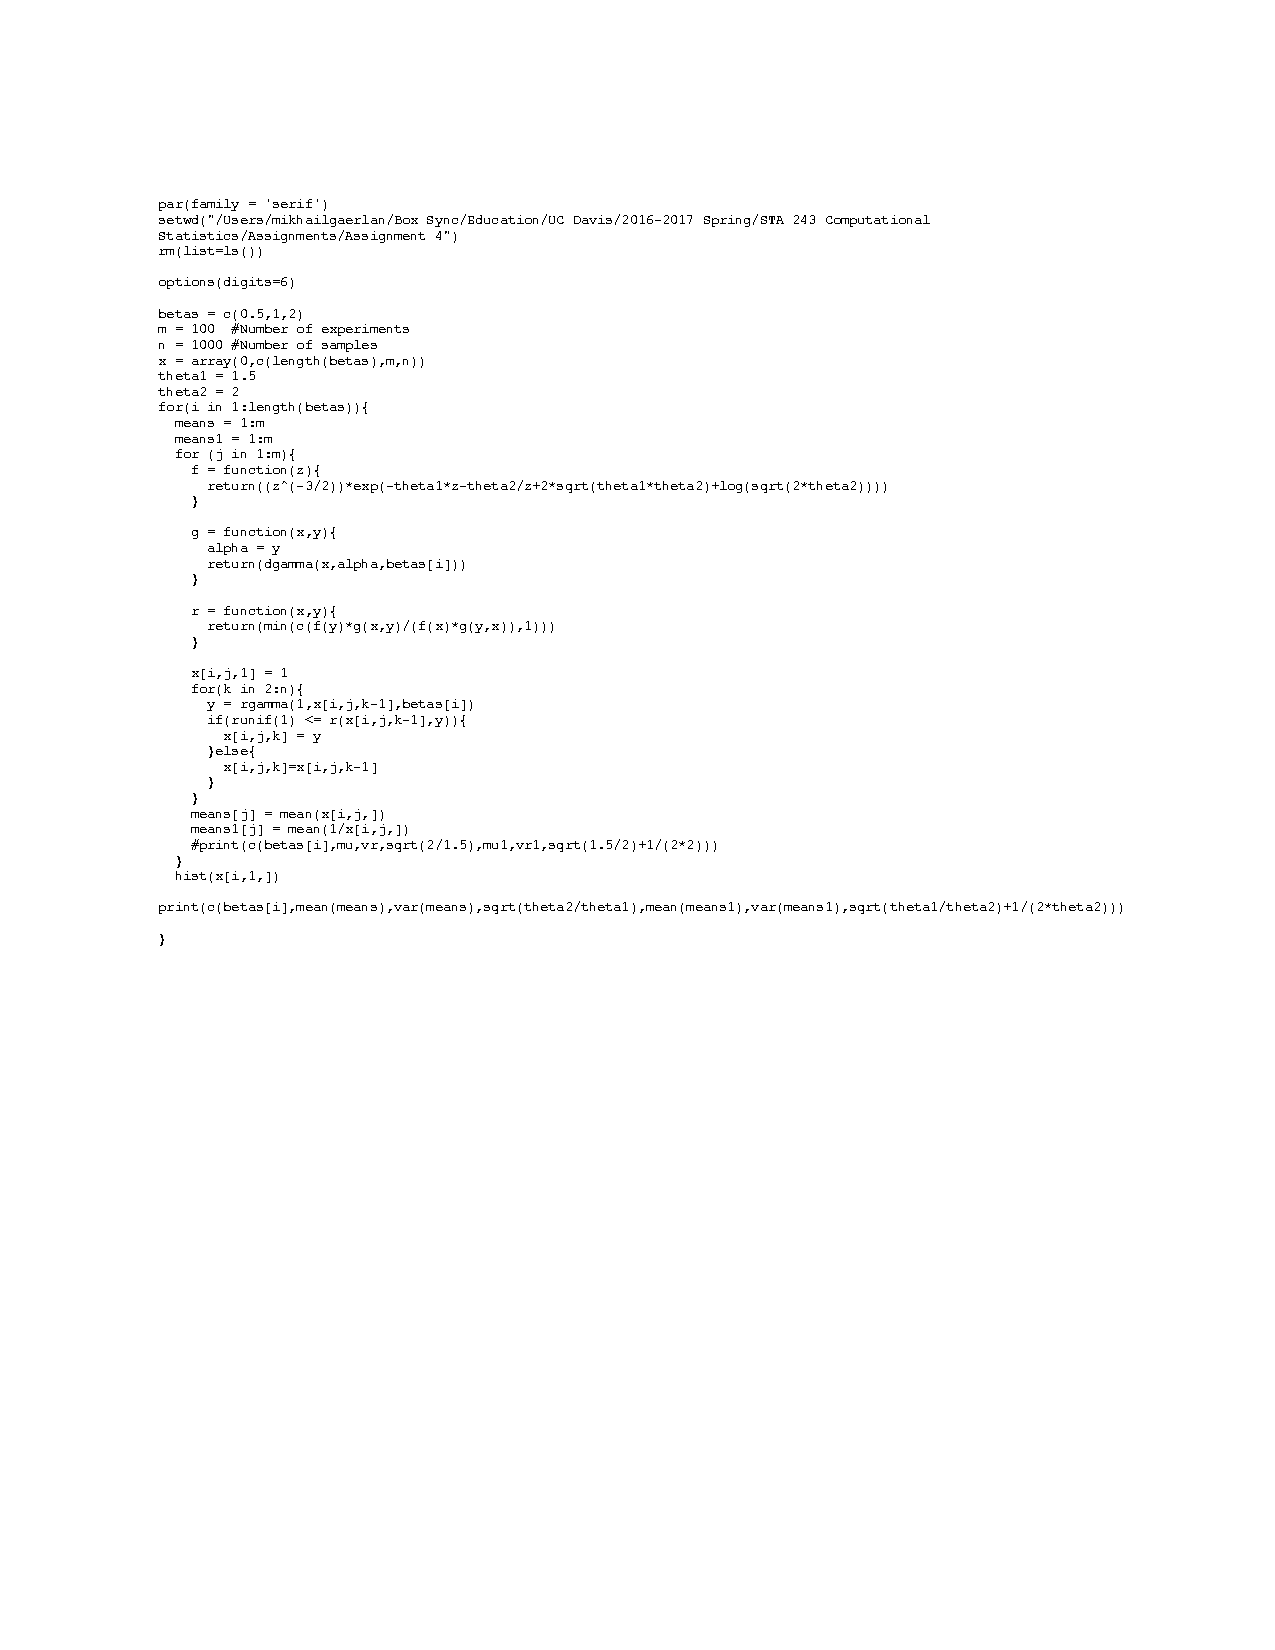
\includepdf[pages={1-1}]{code6.pdf}


\end{document}